% !TeX root = 控制工程基础笔记.tex
\chapter{时域瞬态响应分析}
\label{sec:时域瞬态响应分析}

前一章建立了系统的传递函数模型，把时域微分方程化成了 $s$ 域的代数关系。但要评价一个控制系统「好不好」，最终仍要回到时间域，看它在典型输入下输出的变化过程。本章先给出瞬态响应与稳态响应的概念，然后分别求出一阶系统、二阶系统在典型输入下的解析响应，再由响应曲线引出衡量动态性能的指标，最后说明高阶系统如何用主导极点降阶近似。

\section{时域响应与典型输入信号}
\label{sec:时域响应与典型输入信号}

\begin{definition}[瞬态响应与稳态响应]
系统在某一输入信号作用下，其输出从初始状态变化到稳定状态的过渡过程，称为\textbf{瞬态响应}（又称过渡过程或暂态响应）；当时间趋于无穷大时，系统输出所趋向的最终状态，称为\textbf{稳态响应}。
\end{definition}

\begin{remark}
瞬态响应反映系统的\textbf{动态性能}（快慢、平稳性、超调量），稳态响应反映系统的\textbf{稳态精度}（复现输入的能力）。系统的全响应可看成两部分叠加：一部分由传递函数的极点决定，随 $t\to\infty$ 衰减（或振荡），即瞬态分量；另一部分由输入信号的极点决定，构成稳态分量。因此求时域响应实质上就是求 $X_{\mathrm{o}}(s)=G(s)X_{\mathrm{i}}(s)$ 的拉氏反变换（见附录~\ref{sec:用留数法计算拉氏反变换}）。
\end{remark}

实际输入信号形式繁多，为便于比较与设计，工程上规定了几种典型输入信号，见表~\ref{tab:典型输入信号}。

\begin{table}[H]
\centering
\caption{常用典型输入信号及其象函数}
\label{tab:典型输入信号}
\renewcommand{\arraystretch}{1.5}
\begin{tabular}{cccc}
\toprule
名称 & 时域表达式 $x_{\mathrm{i}}(t)$ & 象函数 $X_{\mathrm{i}}(s)$ & 说明 \\
\midrule
单位脉冲 & $\delta(t)$ & $1$ & 冲击作用，面积恒为 $1$ \\
单位阶跃 & $1(t)$ & $\dfrac{1}{s}$ & 突加常值输入，最常用 \\
单位斜坡 & $t\cdot 1(t)$ & $\dfrac{1}{s^{2}}$ & 随时间匀速增长 \\
单位加速度 & $\dfrac{1}{2}t^{2}\cdot 1(t)$ & $\dfrac{1}{s^{3}}$ & 匀加速输入 \\
正弦 & $A\sin\omega t\cdot 1(t)$ & $\dfrac{A\omega}{s^{2}+\omega^{2}}$ & 频域分析的输入 \\
\bottomrule
\end{tabular}
\end{table}

\begin{tipbox}[为什么用这些典型信号]
单位阶跃信号能暴露系统在突变输入下的超调与调节过程，是最常用、也最容易用实验施加的信号，因此下面主要讨论阶跃响应；单位脉冲信号的响应就是系统的冲激响应 $g(t)$，由卷积定理可知它包含了系统的全部动态信息；单位斜坡信号用于考察系统跟踪匀速输入的能力（稳态误差）。此外，脉冲、阶跃、斜坡、加速度信号之间依次存在微分/积分关系，只需算出一个，其余可通过积分或微分得到，这也是下面推导时的自检手段。
\end{tipbox}

\section{一阶系统的瞬态响应}
\label{sec:一阶系统的瞬态响应}

一阶系统最简单，却包含了指数惯性这一最基本的动态特征。以单位反馈的一阶惯性环节为例，设开环传递函数为 $G(s)=\dfrac{1}{Ts+1}$（$T>0$ 为时间常数），闭环后仍为该形式，于是系统的传递函数为
\begin{equation}
G(s)=\frac{X_{\mathrm{o}}(s)}{X_{\mathrm{i}}(s)}=\frac{1}{Ts+1},
\label{eq:一阶系统传递函数}
\end{equation}
即
\begin{equation}
T\dot{x}_{\mathrm{o}}(t)+x_{\mathrm{o}}(t)=x_{\mathrm{i}}(t),\qquad x_{\mathrm{o}}(0)=0.
\label{eq:一阶系统微分方程}
\end{equation}
下面分别求三种典型输入下的响应。

\subsection{单位阶跃响应}
\label{sec:一阶单位阶跃响应}

输入为单位阶跃 $x_{\mathrm{i}}(t)=1(t)$，其象函数 $X_{\mathrm{i}}(s)=\dfrac{1}{s}$，则输出的象函数为
\begin{equation}
X_{\mathrm{o}}(s)=\frac{1}{Ts+1}\cdot\frac{1}{s}
=\frac{1}{s}-\frac{T}{Ts+1}
=\frac{1}{s}-\frac{1}{s+\dfrac{1}{T}}.
\label{eq:一阶阶跃象函数}
\end{equation}
对式~\eqref{eq:一阶阶跃象函数} 作拉氏反变换，得
\begin{equation}
x_{\mathrm{o}}(t)=\left(1-\mathrm{e}^{-t/T}\right)\cdot 1(t).
\label{eq:一阶阶跃响应}
\end{equation}
响应曲线如图~\ref{fig:一阶系统单位阶跃响应} 所示：曲线从原点出发，以指数规律单调上升，最终趋于稳态值 $1$。

\begin{figure}[H]
\centering
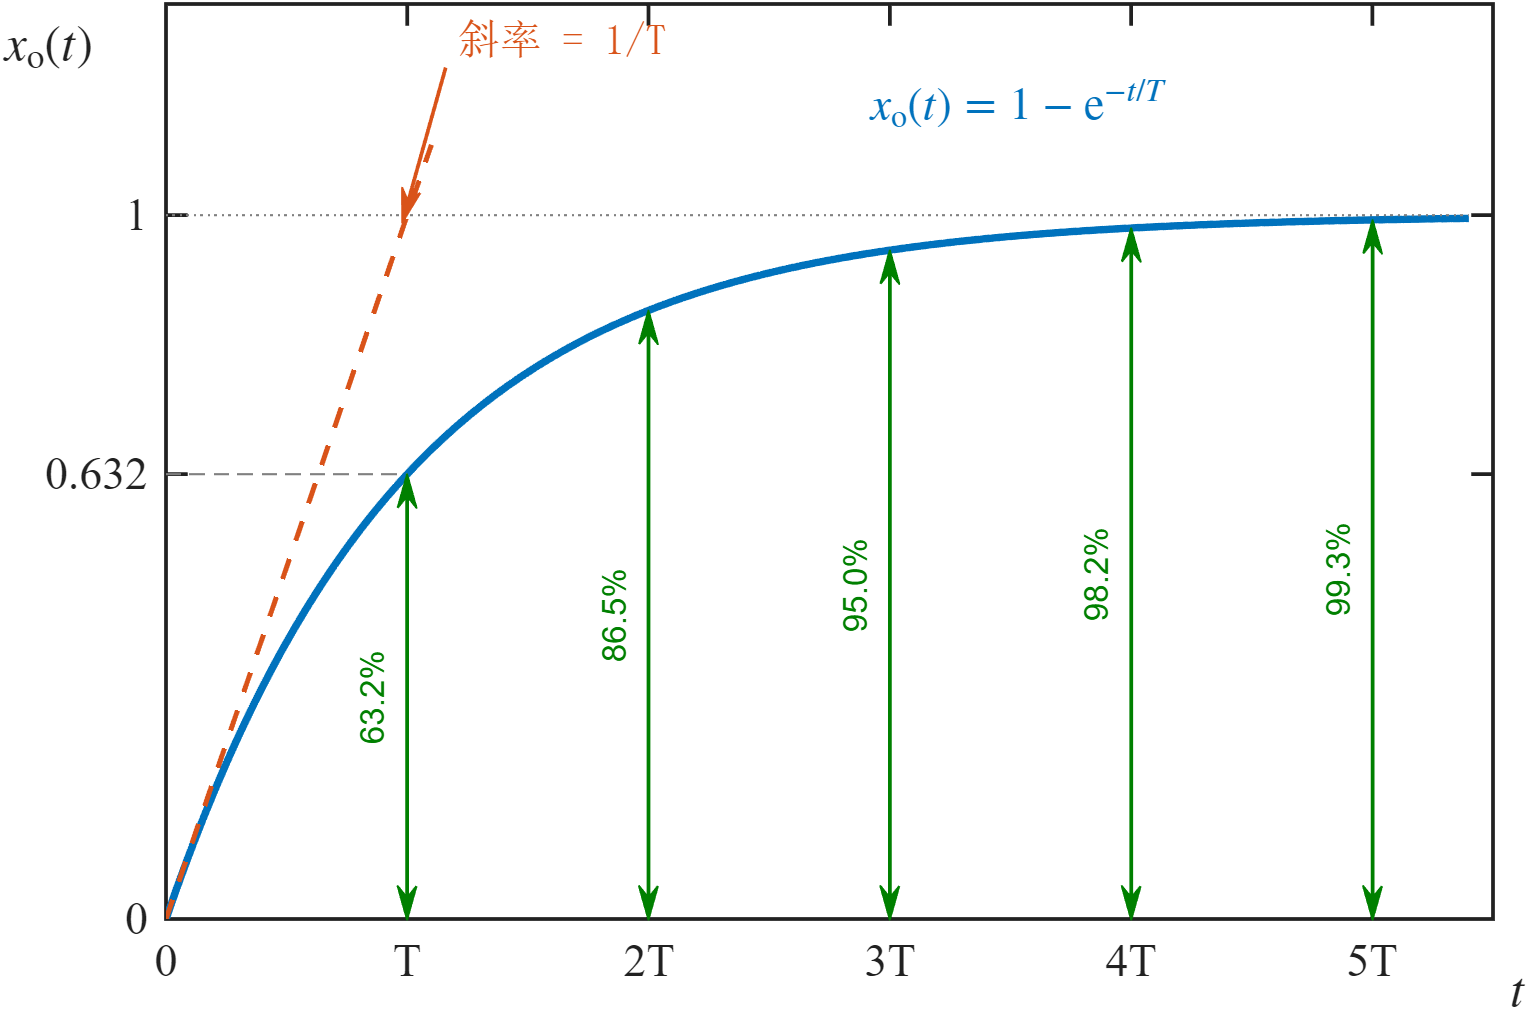
\includegraphics[width=0.82\textwidth]{figures/一阶系统单位阶跃响应.png}
\caption{一阶系统的单位阶跃响应曲线}
\label{fig:一阶系统单位阶跃响应}
\end{figure}

由式~\eqref{eq:一阶阶跃响应} 可直接得到几个常用数值（图~\ref{fig:一阶系统单位阶跃响应} 中已标出）：
\[
t=T:\ 63.2\%,\quad t=2T:\ 86.5\%,\quad t=3T:\ 95.0\%,\quad t=4T:\ 98.2\%,\quad t=5T:\ 99.3\%.
\]

\begin{property}[时间常数的意义]
\begin{itemize}
\item 在 $t=0$ 处对式~\eqref{eq:一阶阶跃响应} 求导，得初始斜率为 $\left.\dfrac{\mathrm{d}x_{\mathrm{o}}}{\mathrm{d}t}\right|_{t=0}=\dfrac{1}{T}$；若按此斜率一直上升，则经过时间 $T$ 恰好达到稳态值。
\item 时间常数 $T$ 是输出上升到稳态值 $63.2\%$ 所需的时间，它是表征系统惯性大小的唯一参数：$T$ 越小，惯性越小，响应越快；$T$ 越大，响应越迟缓。
\item 一阶系统无超调（$M_p=0$）。工程上认为 $t=3T$（误差 $5\%$）到 $t=4T$（误差 $2\%$）时已进入稳态，故一阶系统的调整时间约为 $3T\sim4T$。
\end{itemize}
\end{property}

\subsection{单位斜坡响应}
\label{sec:一阶单位斜坡响应}

输入为单位斜坡 $x_{\mathrm{i}}(t)=t\cdot 1(t)$，其象函数 $X_{\mathrm{i}}(s)=\dfrac{1}{s^{2}}$，则
\begin{equation}
X_{\mathrm{o}}(s)=\frac{1}{Ts+1}\cdot\frac{1}{s^{2}}
=\frac{1}{s^{2}}-\frac{T}{s}+\frac{T}{s+\dfrac{1}{T}}.
\label{eq:一阶斜坡象函数}
\end{equation}
作拉氏反变换，得
\begin{equation}
x_{\mathrm{o}}(t)=\left(t-T+T\mathrm{e}^{-t/T}\right)\cdot 1(t).
\label{eq:一阶斜坡响应}
\end{equation}
记误差 $e(t)=x_{\mathrm{i}}(t)-x_{\mathrm{o}}(t)=T-T\mathrm{e}^{-t/T}$，当 $t\to\infty$ 时
\begin{equation}
e(\infty)=\lim_{t\to\infty}\left(x_{\mathrm{i}}-x_{\mathrm{o}}\right)=T.
\label{eq:一阶斜坡稳态误差}
\end{equation}
响应曲线如图~\ref{fig:一阶系统单位斜坡响应} 所示，可见稳态时输出与输入两条直线平行，但输出滞后了一个恒定的 $T$，即存在大小为 $T$ 的稳态误差。

\begin{figure}[H]
\centering
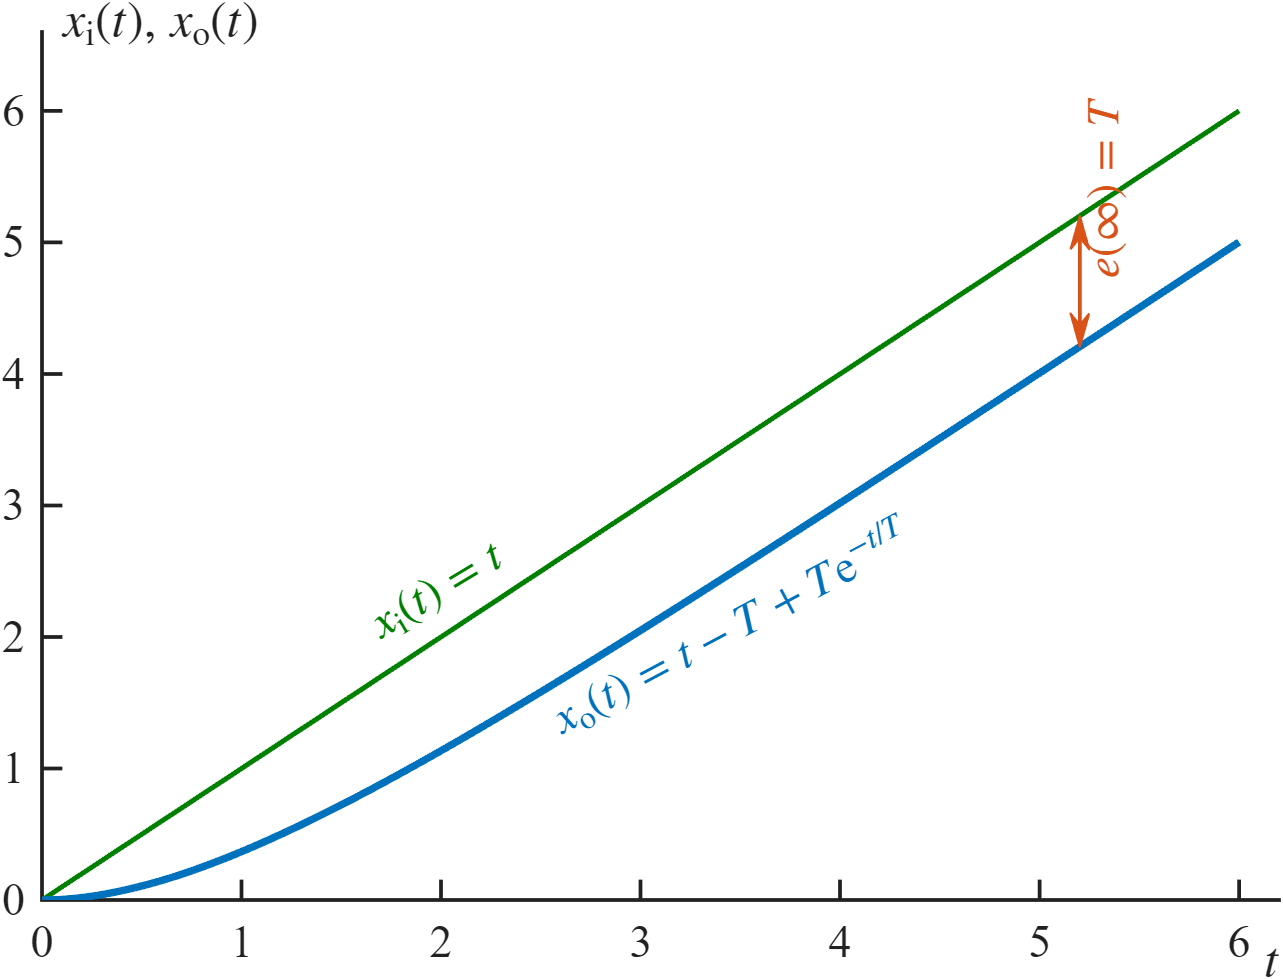
\includegraphics[width=0.72\textwidth]{figures/一阶系统单位斜坡响应.png}
\caption{一阶系统的单位斜坡响应曲线}
\label{fig:一阶系统单位斜坡响应}
\end{figure}

\begin{remark}
由式~\eqref{eq:一阶斜坡稳态误差} 可见，一阶系统跟踪斜坡输入时总有大小为时间常数的稳态误差，且 $T$ 越大误差越大。这说明仅靠一阶惯性环节无法无差地跟踪匀速变化的输入；若要消除该误差，需引入积分环节或提高系统型别。
\end{remark}

\subsection{单位脉冲响应}
\label{sec:一阶单位脉冲响应}

输入为单位脉冲 $x_{\mathrm{i}}(t)=\delta(t)$，其象函数 $X_{\mathrm{i}}(s)=1$，则
\begin{equation}
X_{\mathrm{o}}(s)=\frac{1}{Ts+1}=\frac{1/T}{s+\dfrac{1}{T}}.
\label{eq:一阶脉冲象函数}
\end{equation}
作拉氏反变换，得
\begin{equation}
x_{\mathrm{o}}(t)=\frac{1}{T}\mathrm{e}^{-t/T}\cdot 1(t).
\label{eq:一阶脉冲响应}
\end{equation}
响应曲线如图~\ref{fig:一阶系统单位脉冲响应} 所示，从 $t=0^{+}$ 处的最大值 $\dfrac{1}{T}$ 起按指数规律单调衰减，最终趋于零。

\begin{figure}[H]
\centering
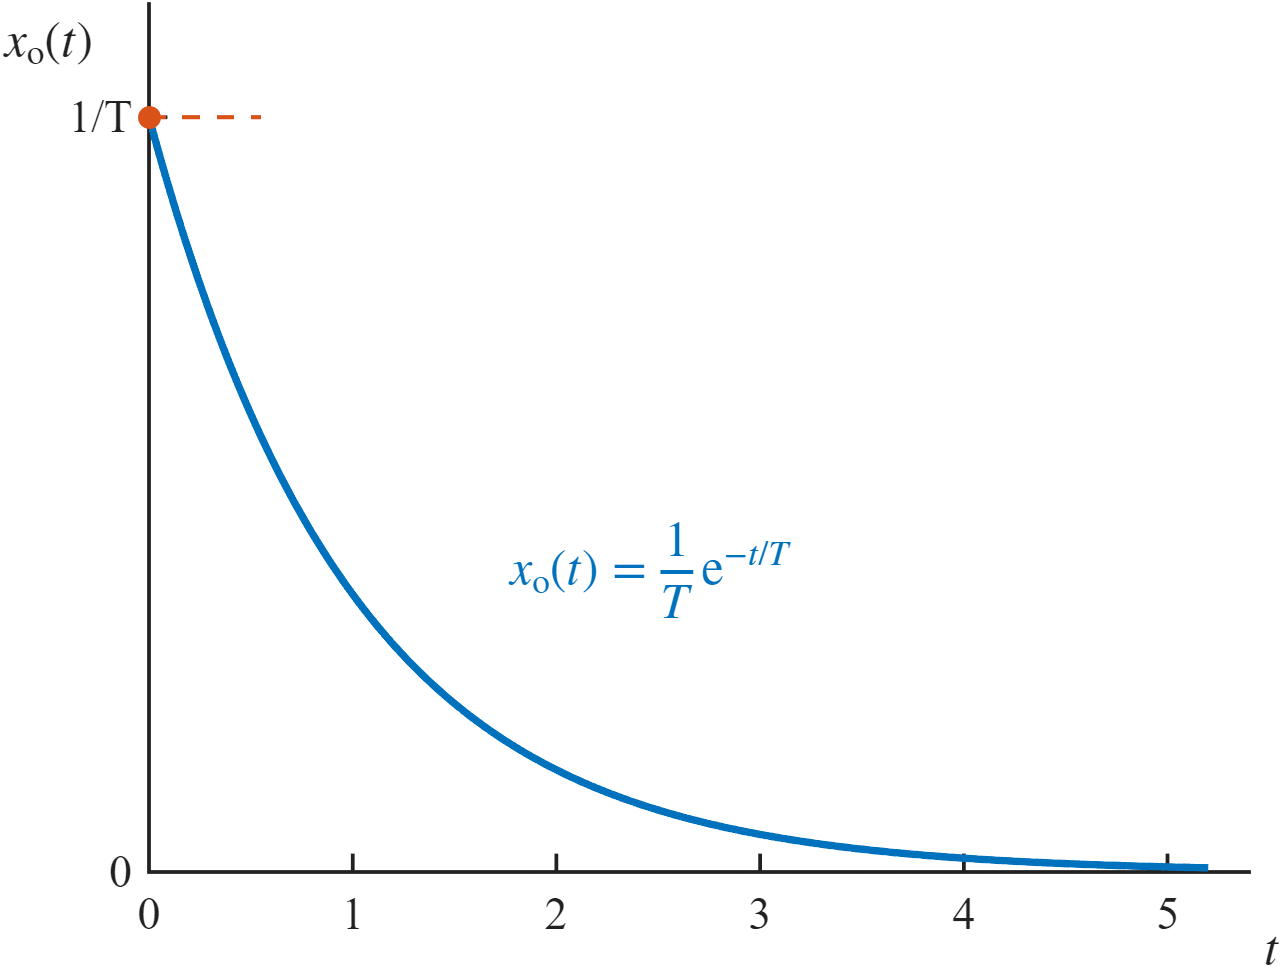
\includegraphics[width=0.62\textwidth]{figures/一阶系统单位脉冲响应.png}
\caption{一阶系统的单位脉冲响应曲线}
\label{fig:一阶系统单位脉冲响应}
\end{figure}

\begin{remark}[三种响应之间的关系]
脉冲、阶跃、斜坡三种输入依次互为积分关系，因而对应的响应也依次互为积分关系：阶跃响应是脉冲响应的积分，斜坡响应又是阶跃响应的积分，
\[
\int_{0}^{t}\frac{1}{T}\mathrm{e}^{-\tau/T}\,\mathrm{d}\tau=1-\mathrm{e}^{-t/T},\qquad
\int_{0}^{t}\left(1-\mathrm{e}^{-\tau/T}\right)\mathrm{d}\tau=t-T+T\mathrm{e}^{-t/T}.
\]
这正与 $X_{\mathrm{i}}(s)$ 中多乘一个 $1/s$ 相对应。算出一个响应后可用此关系校验其余两个。
\end{remark}

\section{二阶系统的瞬态响应}
\label{sec:二阶系统的瞬态响应}

许多实际系统（如质量--弹簧--阻尼系统、RLC 电路、位置随动系统）都可用二阶系统近似描述。将二阶系统写成标准形式
\begin{equation}
G(s)=\frac{X_{\mathrm{o}}(s)}{X_{\mathrm{i}}(s)}
=\frac{\omega_{\mathrm{n}}^{2}}{s^{2}+2\zeta\omega_{\mathrm{n}}s+\omega_{\mathrm{n}}^{2}},
\label{eq:二阶系统标准形式}
\end{equation}
其中 $\omega_{\mathrm{n}}>0$ 为无阻尼自然频率，$\zeta\ge 0$ 为阻尼比。系统的特征方程为
\begin{equation}
s^{2}+2\zeta\omega_{\mathrm{n}}s+\omega_{\mathrm{n}}^{2}=0,
\label{eq:二阶特征方程}
\end{equation}
其两个特征根（极点）为
\begin{equation}
s_{1,2}=-\zeta\omega_{\mathrm{n}}\pm\omega_{\mathrm{n}}\sqrt{\zeta^{2}-1}.
\label{eq:二阶极点}
\end{equation}
极点在复平面上的位置由阻尼比 $\zeta$ 决定，而极点的位置又决定了响应的形状，故按 $\zeta$ 的取值分成四种情形，见表~\ref{tab:阻尼比与响应类型}。

\begin{table}[H]
\centering
\caption{阻尼比与二阶系统的响应类型}
\label{tab:阻尼比与响应类型}
\renewcommand{\arraystretch}{1.5}
\begin{tabular}{cccc}
\toprule
阻尼比 & 极点分布 & 名称 & 阶跃响应形态 \\
\midrule
$\zeta=0$ & 一对纯虚根 $\pm\mathrm{j}\omega_{\mathrm{n}}$ & 无阻尼 & 等幅振荡 \\
$0<\zeta<1$ & 一对共轭复根 $-\zeta\omega_{\mathrm{n}}\pm\mathrm{j}\omega_{\mathrm{d}}$ & 欠阻尼 & 衰减振荡（最常见） \\
$\zeta=1$ & 一对相等负实根 $-\omega_{\mathrm{n}}$ & 临界阻尼 & 单调上升，无超调 \\
$\zeta>1$ & 两个互异负实根 & 过阻尼 & 单调上升，无超调 \\
\bottomrule
\end{tabular}
\end{table}

表中 $\omega_{\mathrm{d}}=\omega_{\mathrm{n}}\sqrt{1-\zeta^{2}}$ 称为\textbf{阻尼振荡角频率}，它是欠阻尼系统实际振荡的角频率；极点实部 $\zeta\omega_{\mathrm{n}}$ 的倒数决定衰减快慢。下面求单位阶跃输入下的响应。

\subsection{欠阻尼情形（$0<\zeta<1$）}
\label{sec:二阶欠阻尼}

此时 $s_{1,2}=-\zeta\omega_{\mathrm{n}}\pm\mathrm{j}\omega_{\mathrm{d}}$，特征方程可写成
\[
\left(s+\zeta\omega_{\mathrm{n}}\right)^{2}+\omega_{\mathrm{d}}^{2}=0,
\qquad
\omega_{\mathrm{d}}=\omega_{\mathrm{n}}\sqrt{1-\zeta^{2}}.
\]
单位阶跃输入的象函数为 $X_{\mathrm{i}}(s)=\dfrac{1}{s}$，代入式~\eqref{eq:二阶系统标准形式} 并用留数法（或部分分式）求反变换，得
\begin{equation}
x_{\mathrm{o}}(t)=\left[1-\frac{\mathrm{e}^{-\zeta\omega_{\mathrm{n}}t}}{\sqrt{1-\zeta^{2}}}
\sin\left(\omega_{\mathrm{d}}t+\beta\right)\right]\cdot 1(t),
\label{eq:二阶欠阻尼阶跃响应}
\end{equation}
其中
\begin{equation}
\beta=\arctan\frac{\sqrt{1-\zeta^{2}}}{\zeta}=\arccos\zeta.
\label{eq:beta}
\end{equation}
式~\eqref{eq:二阶欠阻尼阶跃响应} 表明：欠阻尼二阶系统的阶跃响应由稳态分量 $1$ 和衰减振荡分量两部分组成，包络 $\mathrm{e}^{-\zeta\omega_{\mathrm{n}}t}$ 决定衰减快慢，$\omega_{\mathrm{d}}$ 决定振荡频率。$\zeta$ 越小，振荡越剧烈、超调越大。

\subsection{临界阻尼情形（$\zeta=1$）}
\label{sec:二阶临界阻尼}

此时 $s_{1}=s_{2}=-\omega_{\mathrm{n}}$ 为二重实根，传递函数为
\[
G(s)=\frac{\omega_{\mathrm{n}}^{2}}{\left(s+\omega_{\mathrm{n}}\right)^{2}}.
\]
单位阶跃响应为（推导同附录例~\ref{exam:重极点}）
\begin{equation}
x_{\mathrm{o}}(t)=\left[1-\left(1+\omega_{\mathrm{n}}t\right)\mathrm{e}^{-\omega_{\mathrm{n}}t}\right]\cdot 1(t).
\label{eq:二阶临界阻尼阶跃响应}
\end{equation}
响应单调上升且无超调，是所有不超过稳态值的响应中过渡过程最短的一种。

\subsection{过阻尼情形（$\zeta>1$）}
\label{sec:二阶过阻尼}

此时式~\eqref{eq:二阶极点} 给出两个互异的负实根，可记
\[
s_{1}=-\zeta\omega_{\mathrm{n}}+\omega_{\mathrm{n}}\sqrt{\zeta^{2}-1}<0,\qquad
s_{2}=-\zeta\omega_{\mathrm{n}}-\omega_{\mathrm{n}}\sqrt{\zeta^{2}-1}<0,
\qquad s_{1}s_{2}=\omega_{\mathrm{n}}^{2}.
\]
单位阶跃响应为
\begin{equation}
x_{\mathrm{o}}(t)=\left[1+\frac{\omega_{\mathrm{n}}}{2\sqrt{\zeta^{2}-1}}
\left(\frac{\mathrm{e}^{s_{1}t}}{s_{1}}-\frac{\mathrm{e}^{s_{2}t}}{s_{2}}\right)\right]\cdot 1(t).
\label{eq:二阶过阻尼阶跃响应}
\end{equation}
由于 $s_{1}$、$s_{2}$ 都位于负实轴上，两个瞬态分量都是单调衰减的指数项，故响应单调上升、无超调。

\begin{remark}
过阻尼响应是两个一阶惯性环节串联的结果，其中时间常数大（离虚轴近）的那个极点主导了过渡过程，另一个极点的影响很快消失。当 $\zeta\gg1$ 时，系统响应缓慢；工程上一般不取过阻尼，而取 $\zeta=0.4\sim0.8$ 的欠阻尼状态，在快速性与平稳性之间折中。
\end{remark}

\section{二阶系统的时域性能指标}
\label{sec:二阶系统时域性能指标}

工程上并不逐点比较响应曲线，而是用几个特征量描述动态性能。这些指标通常在单位阶跃响应曲线上定义，如图~\ref{fig:二阶系统时域性能指标} 所示。

\begin{figure}[H]
\centering
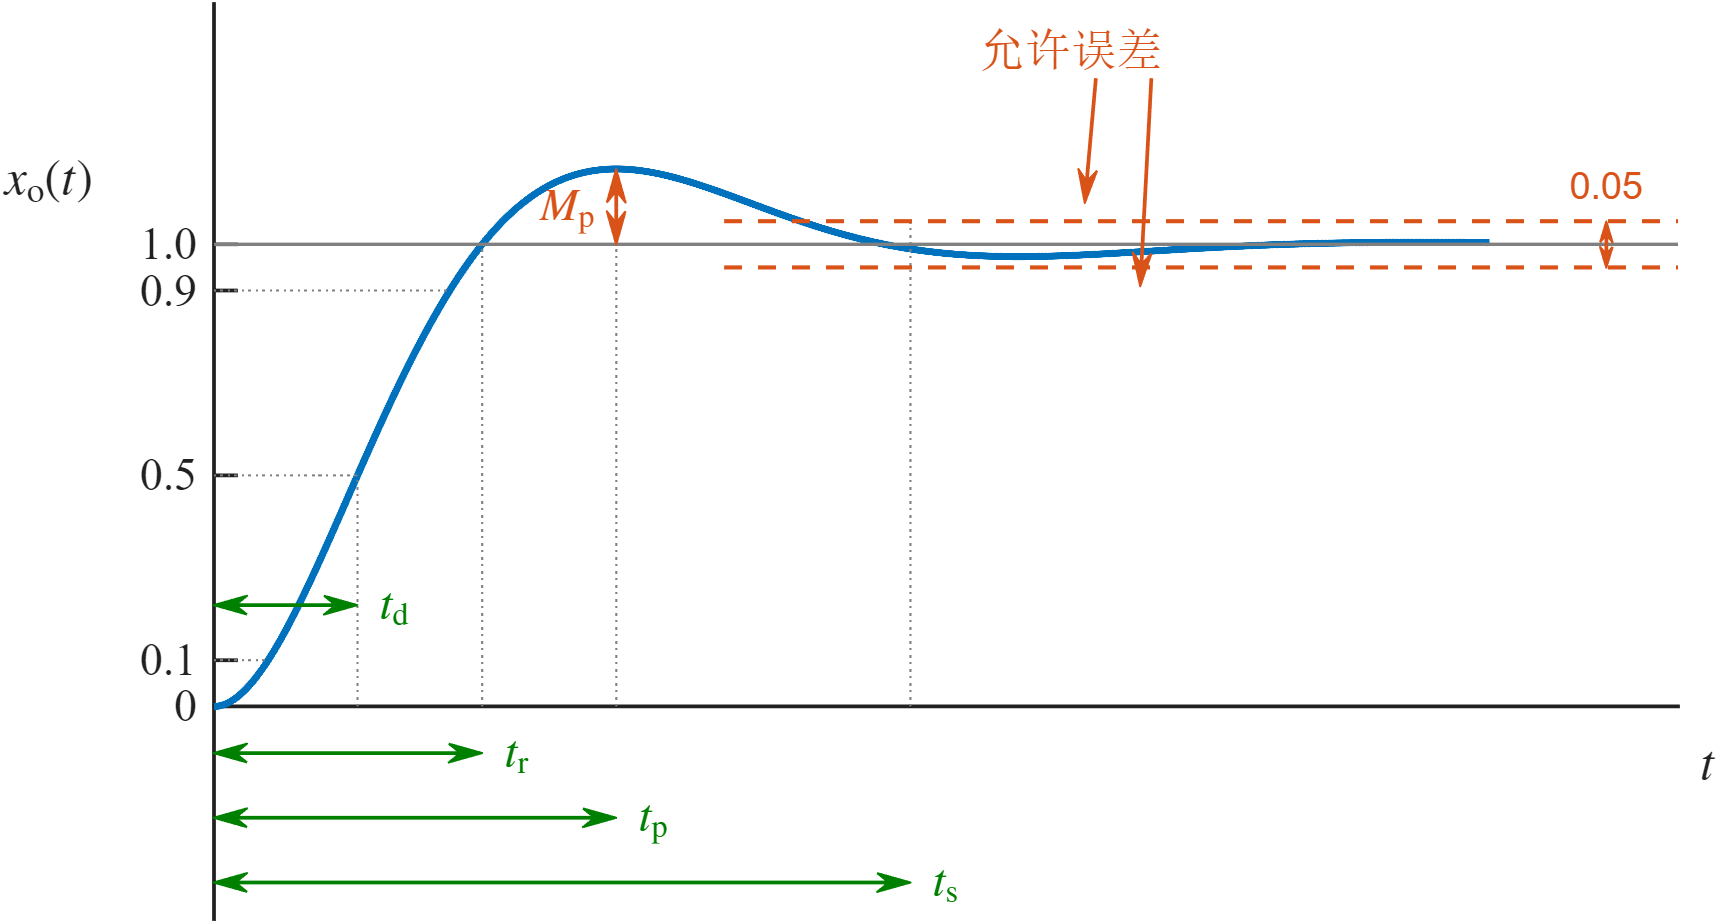
\includegraphics[width=0.82\textwidth]{figures/二阶系统时域性能指标.png}
\caption{二阶系统单位阶跃响应的时域性能指标}
\label{fig:二阶系统时域性能指标}
\end{figure}

\subsection{上升时间 $t_{\mathrm{r}}$}
\label{sec:上升时间}

\textbf{上升时间}指响应曲线从零时刻首次到达稳态值所需的时间。对欠阻尼系统，令式~\eqref{eq:二阶欠阻尼阶跃响应} 中 $x_{\mathrm{o}}(t_{\mathrm{r}})=1$，即
\[
\sin\left(\omega_{\mathrm{d}}t_{\mathrm{r}}+\beta\right)=0,
\]
取第一个正根
\begin{equation}
\omega_{\mathrm{d}}t_{\mathrm{r}}+\beta=\pi,
\qquad\Longrightarrow\qquad
t_{\mathrm{r}}=\frac{\pi-\beta}{\omega_{\mathrm{d}}},
\label{eq:上升时间}
\end{equation}
其中 $\beta$ 由式~\eqref{eq:beta} 给出。

\begin{remark}
对无超调的系统，响应理论上要到 $t\to\infty$ 才严格到达稳态值，故此时改用「从稳态值的 $10\%$ 上升到 $90\%$ 所需的时间」作为上升时间。
\end{remark}

\subsection{峰值时间 $t_{\mathrm{p}}$ 与最大超调量 $M_{\mathrm{p}}$}
\label{sec:峰值时间与超调}

\textbf{峰值时间}指响应曲线第一次到达峰值所需的时间。峰值点处导数为零，令 $\dfrac{\mathrm{d}x_{\mathrm{o}}(t)}{\mathrm{d}t}=0$，由式~\eqref{eq:二阶欠阻尼阶跃响应} 得
\begin{equation}
\frac{\zeta\omega_{\mathrm{n}}\mathrm{e}^{-\zeta\omega_{\mathrm{n}}t_{\mathrm{p}}}}{\sqrt{1-\zeta^{2}}}
\sin\left(\omega_{\mathrm{d}}t_{\mathrm{p}}+\beta\right)
-\frac{\omega_{\mathrm{d}}\mathrm{e}^{-\zeta\omega_{\mathrm{n}}t_{\mathrm{p}}}}{\sqrt{1-\zeta^{2}}}
\cos\left(\omega_{\mathrm{d}}t_{\mathrm{p}}+\beta\right)=0.
\label{eq:峰值条件}
\end{equation}
因 $\mathrm{e}^{-\zeta\omega_{\mathrm{n}}t_{\mathrm{p}}}\neq0$，式~\eqref{eq:峰值条件} 化为
\[
\tan\left(\omega_{\mathrm{d}}t_{\mathrm{p}}+\beta\right)=\frac{\omega_{\mathrm{d}}}{\zeta\omega_{\mathrm{n}}}=\tan\beta,
\]
取第一个正根即得
\begin{equation}
t_{\mathrm{p}}=\frac{\pi}{\omega_{\mathrm{d}}}=\frac{\pi}{\omega_{\mathrm{n}}\sqrt{1-\zeta^{2}}}.
\label{eq:峰值时间}
\end{equation}

\textbf{最大超调量}指响应曲线的最大峰值与稳态值之差，通常用百分数表示：
\begin{equation}
M_{\mathrm{p}}=x_{\mathrm{o}}\left(t_{\mathrm{p}}\right)-x_{\mathrm{o}}(\infty),
\qquad
M_{\mathrm{p}}\%=\frac{x_{\mathrm{o}}\left(t_{\mathrm{p}}\right)-x_{\mathrm{o}}(\infty)}{x_{\mathrm{o}}(\infty)}\times100\%.
\label{eq:超调量定义}
\end{equation}
将式~\eqref{eq:峰值时间} 代入式~\eqref{eq:二阶欠阻尼阶跃响应}，并注意 $\sin(\pi+\beta)=-\sin\beta=-\sqrt{1-\zeta^{2}}$，得
\begin{equation}
M_{\mathrm{p}}=\mathrm{e}^{-\pi\zeta/\sqrt{1-\zeta^{2}}},
\qquad
M_{\mathrm{p}}\%=\mathrm{e}^{-\pi\zeta/\sqrt{1-\zeta^{2}}}\times100\%.
\label{eq:超调量}
\end{equation}

\begin{keybox}[超调量只与阻尼比有关]
由式~\eqref{eq:超调量} 可见，$M_{\mathrm{p}}$ 仅是阻尼比 $\zeta$ 的函数，与 $\omega_{\mathrm{n}}$ 无关；$\zeta$ 越小，超调越大。因此若只希望改变超调量，应调整阻尼比；而改变 $\omega_{\mathrm{n}}$ 只能改变响应快慢，不影响超调量。
\end{keybox}

\subsection{延迟时间 $t_{\mathrm{d}}$}
\label{sec:延迟时间}

\textbf{延迟时间}指响应曲线从零上升到稳态值 $50\%$ 所需要的时间。$t_{\mathrm{d}}$ 没有简单的解析表达式，工程上常用下列经验近似：
\begin{equation}
t_{\mathrm{d}}\approx\frac{1+0.7\zeta}{\omega_{\mathrm{n}}}.
\label{eq:延迟时间}
\end{equation}
由式可见，$\omega_{\mathrm{n}}$ 越大、$\zeta$ 越小，延迟时间越短。

\subsection{调整时间 $t_{\mathrm{s}}$}
\label{sec:调整时间}

\textbf{调整时间}指响应曲线进入并一直保持在允许误差范围（通常取稳态值的 $\pm5\%$ 或 $\pm2\%$，也写作 $0.05$ 或 $0.02$）内的最短时间。它的求解借助响应的\textbf{包络线}
\begin{equation}
F(t)=1\pm\frac{\mathrm{e}^{-\zeta\omega_{\mathrm{n}}t}}{\sqrt{1-\zeta^{2}}}.
\label{eq:响应包络线}
\end{equation}
包络线以内是响应曲线，只要包络线进入误差带，响应也必然进入。以 $\pm5\%$ 误差带为例，令
\[
\frac{\mathrm{e}^{-\zeta\omega_{\mathrm{n}}t_{\mathrm{s}}}}{\sqrt{1-\zeta^{2}}}=0.05,
\]
解得
\begin{equation}
t_{\mathrm{s}}=\frac{-\ln 0.05-\ln\sqrt{1-\zeta^{2}}}{\zeta\omega_{\mathrm{n}}}.
\label{eq:调整时间精确}
\end{equation}
当阻尼比 $\zeta$ 较小时，$\ln\sqrt{1-\zeta^{2}}$ 相对 $-\ln 0.05=\ln20\approx3$ 可忽略，于是
\begin{equation}
t_{\mathrm{s}}\approx\frac{-\ln 0.05}{\zeta\omega_{\mathrm{n}}}=\frac{\ln20}{\zeta\omega_{\mathrm{n}}}\approx\frac{3}{\zeta\omega_{\mathrm{n}}}
\qquad(\pm2\%:\ t_{\mathrm{s}}\approx\frac{4}{\zeta\omega_{\mathrm{n}}}).
\label{eq:调整时间近似}
\end{equation}
即调整时间与 $\zeta\omega_{\mathrm{n}}$ 成反比；$\zeta\omega_{\mathrm{n}}$ 越大，衰减越快，过渡过程越短。

\subsection{振荡次数 $N$}
\label{sec:振荡次数}

\textbf{振荡次数}指在调整时间 $t_{\mathrm{s}}$ 内响应曲线穿越稳态值（或在误差带内）的振荡周期数。振荡周期 $T_{\mathrm{d}}=\dfrac{2\pi}{\omega_{\mathrm{d}}}$，结合式~\eqref{eq:调整时间近似} 得
\begin{equation}
N=\frac{t_{\mathrm{s}}}{T_{\mathrm{d}}}=\frac{t_{\mathrm{s}}\omega_{\mathrm{d}}}{2\pi}
\approx\frac{3\sqrt{1-\zeta^{2}}}{2\pi\zeta}
\qquad(\pm5\%\text{ 误差带}).
\label{eq:振荡次数}
\end{equation}

\begin{keybox}[时域性能指标小结]
\centering
\renewcommand{\arraystretch}{1.6}
\begin{tabular}{lll}
\toprule
指标 & 定义 & 近似计算 \\
\midrule
上升时间 $t_{\mathrm{r}}$ & 首次到达稳态值的时间 & $\dfrac{\pi-\beta}{\omega_{\mathrm{d}}}$ \\
峰值时间 $t_{\mathrm{p}}$ & 首次到达峰值的时间 & $\dfrac{\pi}{\omega_{\mathrm{d}}}$ \\
最大超调量 $M_{\mathrm{p}}$ & 峰值与稳态值之差（百分数） & $\mathrm{e}^{-\pi\zeta/\sqrt{1-\zeta^{2}}}$ \\
延迟时间 $t_{\mathrm{d}}$ & 上升到稳态值 $50\%$ 的时间 & $\dfrac{1+0.7\zeta}{\omega_{\mathrm{n}}}$ \\
调整时间 $t_{\mathrm{s}}$ & 进入 $\pm5\%$（或 $\pm2\%$）误差带的时间 & $\dfrac{3}{\zeta\omega_{\mathrm{n}}}$（或 $\dfrac{4}{\zeta\omega_{\mathrm{n}}}$） \\
振荡次数 $N$ & 调整时间内振荡的周期数 & $\dfrac{3\sqrt{1-\zeta^{2}}}{2\pi\zeta}$ \\
\bottomrule
\end{tabular}
\end{keybox}

\begin{remark}
六个指标可分为两类：$M_{\mathrm{p}}$ 与 $N$ 只由 $\zeta$ 决定，反映\textbf{相对稳定性}；$t_{\mathrm{r}}$、$t_{\mathrm{p}}$、$t_{\mathrm{d}}$、$t_{\mathrm{s}}$ 由 $\zeta$ 与 $\omega_{\mathrm{n}}$ 共同决定，反映响应的\textbf{快速性}。减小 $\zeta$ 可缩短上升时间，但超调与振荡次数增大；提高 $\omega_{\mathrm{n}}$ 则各项时间指标都缩短而超调不变。设计时正是通过调整这两个参数取得动态性能的折中。
\end{remark}

\section{高阶系统的瞬态响应}
\label{sec:高阶系统的瞬态响应}

设高阶线性定常系统的传递函数为
\begin{equation}
\frac{X_{\mathrm{o}}(s)}{X_{\mathrm{i}}(s)}
=\frac{k\left(s^{m}+b_{1}s^{m-1}+\cdots+b_{m-1}s+b_{m}\right)}{s^{n}+a_{1}s^{n-1}+\cdots+a_{n-1}s+a_{n}}
=\frac{k\prod_{i=1}^{m}\left(s+z_{i}\right)}
{\prod_{j=1}^{q}\left(s+p_{j}\right)\prod_{k=1}^{r}\left(s^{2}+2\zeta_{k}\omega_{k}s+\omega_{k}^{2}\right)},
\label{eq:高阶传递函数}
\end{equation}
其中 $q$ 个为实极点、$2r$ 个为共轭复极点，$q+2r=n$，且 $m\le n$。在单位阶跃输入 $X_{\mathrm{i}}(s)=\dfrac{1}{s}$ 下
\begin{equation}
X_{\mathrm{o}}(s)=\frac{k\left(s^{m}+b_{1}s^{m-1}+\cdots+b_{m}\right)}
{s\prod_{j=1}^{q}\left(s+p_{j}\right)\prod_{k=1}^{r}\left(s^{2}+2\zeta_{k}\omega_{k}s+\omega_{k}^{2}\right)}.
\label{eq:高阶阶跃象函数}
\end{equation}
若各极点互不相同，式~\eqref{eq:高阶阶跃象函数} 可展成部分分式
\begin{equation}
X_{\mathrm{o}}(s)=\frac{\alpha}{s}+\sum_{j=1}^{q}\frac{\alpha_{j}}{s+p_{j}}
+\sum_{k=1}^{r}\frac{\beta_{k}\left(s+\zeta_{k}\omega_{k}\right)+\gamma_{k}\omega_{k}\sqrt{1-\zeta_{k}^{2}}}
{\left(s+\zeta_{k}\omega_{k}\right)^{2}+\left(\omega_{k}\sqrt{1-\zeta_{k}^{2}}\right)^{2}},
\label{eq:高阶部分分式}
\end{equation}
作拉氏反变换，得时域响应
\begin{equation}
\begin{aligned}
x_{\mathrm{o}}(t)=\ & \alpha+\sum_{j=1}^{q}\alpha_{j}\mathrm{e}^{-p_{j}t}
+\sum_{k=1}^{r}\beta_{k}\mathrm{e}^{-\zeta_{k}\omega_{k}t}\cos\left(\omega_{k}\sqrt{1-\zeta_{k}^{2}}\right)t\\
& +\sum_{k=1}^{r}\gamma_{k}\mathrm{e}^{-\zeta_{k}\omega_{k}t}\sin\left(\omega_{k}\sqrt{1-\zeta_{k}^{2}}\right)t.
\end{aligned}
\label{eq:高阶时域响应}
\end{equation}
可见高阶系统的响应是一系列一阶、二阶分量的叠加，其中 $\alpha$ 为稳态分量，各指数项和衰减振荡项为瞬态分量。

\subsection{主导极点与偶极子相消}
\label{sec:主导极点}

直接按式~\eqref{eq:高阶时域响应} 分析高阶系统过于繁琐，工程上常用下面的规则降阶近似：

\begin{keybox}[高阶系统简化的两条规则]
\begin{enumerate}
\item \textbf{主导极点}：离虚轴最近、且其留数（系数）不为零的极点，其对应的瞬态分量衰减最慢、在响应中占主导地位，称为主导极点。若其他极点的实部比主导极点的实部大 $5$ 倍以上，这些极点对应的分量的衰减速度快得多，且通常留数也小，可忽略不计。
\item \textbf{偶极子相消}：若某零点与某极点相距很近（组成一对偶极子），则它们对应的瞬态分量系数近似为零，该零点与该极点近似相消，可同时略去。
\end{enumerate}
\end{keybox}

\begin{tipbox}[处理方法]
用主导极点降阶的一般做法是：
\begin{enumerate}
\item 把传递函数化为「首一式」形式，即使各因子的常数项为 $1$，便于比较极点与零点离虚轴的远近；
\item 找出主导极点，忽略次要极点（以及离虚轴很近、可与极点相消的零点），把系统降为一阶或二阶系统；
\item 令降阶后的近似模型与原系统\textbf{静态增益相同}，以确定近似模型的系数。
\end{enumerate}
\end{tipbox}

\begin{longexample}[用主导极点降阶近似]
\label{exam:主导极点降阶}
设某高阶系统的传递函数为
\[
G(s)=\frac{0.2s+1}{\left(s+0.2\right)\left(s+1\right)\left(s+10\right)}.
\]
试用主导极点法将其降为一阶近似，并写出近似传递函数。
\begin{solution}
\textbf{（1）化为首一式并确定极点、零点。} 分子 $0.2s+1=0.2\left(s+5\right)$，含零点 $s=-5$；分母含极点 $s=-0.2$、$s=-1$、$s=-10$。

\textbf{（2）判断主导极点。} 三个极点离虚轴的距离（实部绝对值）分别为 $0.2$、$1$、$10$。最近的是 $s=-0.2$，其次是 $s=-1$，二者相距 $5$ 倍，$s=-10$ 则远得多。故 $s=-0.2$ 为\textbf{主导极点}，$s=-1$、$s=-10$ 可略去；零点 $s=-5$ 与任一极点都不构成偶极子，一并略去。

\textbf{（3）确定近似模型的系数。} 原系统的静态增益为
\[
G(0)=\frac{1}{0.2\times1\times10}=0.5.
\]
设降阶后的一阶模型为 $\dfrac{K}{Ts+1}$，其中主导极点为 $s=-0.2$，故时间常数 $T=\dfrac{1}{0.2}=5$。再令近似模型与原系统静态增益相同，$G(0)=K=0.5$，得
\[
G(s)\approx\frac{0.5}{5s+1}=\frac{0.1}{s+0.2}.
\]
即该高阶系统可用一个放大系数为 $0.5$、时间常数为 $5$ 的一阶惯性环节近似描述，其瞬态响应可直接查表~\ref{tab:常用拉氏变换对}（或用式~\eqref{eq:一阶阶跃响应}）得到。
\end{solution}
\end{longexample}

\begin{remark}
主导极点法是「抓主要矛盾」的思想：离虚轴最近、衰减最慢的分量决定了过渡过程的大部分形态。它把高阶系统化简为一阶或二阶系统，从而可以套用本章前面的一阶、二阶结论估算性能指标，非常便于工程初步设计。当然，被忽略的极点会在过渡过程刚开始的短时内造成一定误差，若要求精确结果仍需回到原传递函数求解。
\end{remark}
